% ATLAS: setting up the Station PC -- a run-book for the Windows PC with the RTX 5070.
% Written by hand; compile with pdflatex. Facts come from the Master Plan (Appendix C.7, section 7,
% Appendix B.4) and from the vendors' own pages, package indexes and source files, read on 3 October 2026.
\documentclass[10pt]{article}
\usepackage[a4paper,top=13mm,bottom=17mm,left=16mm,right=16mm,footskip=9mm]{geometry}
\usepackage[T1]{fontenc}
\usepackage[utf8]{inputenc}
\input{glyphtounicode}\pdfgentounicode=1
\usepackage{helvet}
\renewcommand{\familydefault}{\sfdefault}
\usepackage[varqu,varl]{zi4}
\usepackage[table]{xcolor}
\usepackage{array,booktabs,ragged2e,multicol}
\usepackage{enumitem}
\usepackage{needspace}
\usepackage{listings}
\usepackage{tikz}
\usetikzlibrary{positioning,fit,calc}

\pdfinfo{/Title (ATLAS: setting up the Station PC)}

% ---------- colours (the palette of the other ATLAS handouts) ----------
\definecolor{ink}{HTML}{1F2933}
\definecolor{mute}{HTML}{56616B}
\definecolor{laneC}{HTML}{FDEEDE}
\definecolor{laneD}{HTML}{E3EDFC}
\definecolor{headC}{HTML}{F9D6B2}
\definecolor{headD}{HTML}{C5D9F8}
\definecolor{accC}{HTML}{9A4A00}
\definecolor{accD}{HTML}{1B55B0}
\definecolor{cmdbg}{HTML}{F1F3F5}
\definecolor{rule}{HTML}{CBD2D9}
\definecolor{trapbg}{HTML}{FDF3E7}
\definecolor{laterbg}{HTML}{EEF2F6}
\definecolor{admin}{HTML}{A61B1B}

% ---------- footer ----------
\makeatletter
\def\ps@atlas{%
  \def\@oddhead{}\def\@evenhead{}%
  \def\@oddfoot{\parbox{\textwidth}{\footnotesize\color{mute}ATLAS: setting up the Station PC\hfill 3 October 2026\hspace{6mm}Page \thepage}}%
  \let\@evenfoot\@oddfoot}
\makeatother
\pagestyle{atlas}

\setlength{\parindent}{0pt}
\setlength{\parskip}{0pt}
\color{ink}

% ---------- commands to type, and what they print ----------
% Commands are set so that copying them out of the PDF gives exactly what is printed:
% plain ASCII quotes and hyphens, one command per line, no prompt characters, no wrapped lines.
\lstdefinestyle{cmd}{basicstyle=\ttfamily\fontsize{8.35}{11.3}\selectfont\color{ink},columns=fullflexible,
  keepspaces=true,upquote=true,showstringspaces=false,backgroundcolor=\color{cmdbg},frame=none,
  aboveskip=3.5pt,belowskip=3.5pt,xleftmargin=6pt,framexleftmargin=6pt,breaklines=false}
\lstdefinestyle{out}{basicstyle=\ttfamily\fontsize{8.2}{10.6}\selectfont\color{mute},columns=fullflexible,
  keepspaces=true,upquote=true,showstringspaces=false,frame=leftline,framerule=1.2pt,rulecolor=\color{rule},
  aboveskip=2.5pt,belowskip=3.5pt,xleftmargin=7pt,framexleftmargin=5pt,breaklines=false}
\lstdefinestyle{inl}{basicstyle=\ttfamily\fontsize{8.8}{11}\selectfont,columns=fullflexible,keepspaces=true,
  upquote=true,showstringspaces=false,breaklines=true}
\lstnewenvironment{cmd}{\lstset{style=cmd}}{}
\lstnewenvironment{out}{\lstset{style=out}}{}
\newcommand{\cc}{\lstinline[style=inl]}
\newcommand{\code}[1]{{\ttfamily\fontsize{8.8}{11}\selectfont #1}}

% where a block is typed, when it is not a normal PowerShell window
\newcommand{\tagchip}[2]{{\setlength{\fboxsep}{1.6pt}\colorbox{#1}{\fontsize{6.6}{8}\selectfont\bfseries\color{white}\,#2\,}}}
\newcommand{\asadmin}{\tagchip{admin}{ADMINISTRATOR}\enskip}
\newcommand{\onphone}{\tagchip{accC}{ON EACH PHONE}\enskip}
\newcommand{\see}{\par\vspace{0.6mm}{\footnotesize\color{mute}You should see:}}

% ---------- parts and steps ----------
\newcounter{partno}
% \Part{title}{what is true when the part is done}
\newcommand{\Part}[2]{%
  \par\vspace{6mm}\needspace{42mm}\refstepcounter{partno}%
  {\setlength{\fboxsep}{0pt}\colorbox{laneD}{\parbox{\linewidth}{\vspace{2.2mm}\hspace{3mm}%
    {\fontsize{17}{19}\selectfont\bfseries\color{accD}\thepartno}\hspace{3mm}%
    {\fontsize{13.5}{16}\selectfont\bfseries\color{ink}#1}\vspace{2.2mm}}}}\par\nopagebreak
  \if\relax\detokenize{#2}\relax\vspace{2.4mm}\else
  \vspace{1.8mm}{\small\color{mute}\textbf{Done when:} #2\par}\nopagebreak\vspace{1.4mm}\fi}
\newlist{steps}{enumerate}{1}
\setlist[steps]{label=\textbf{\thepartno.\arabic*},leftmargin=9.5mm,labelsep=2.5mm,itemsep=2.8mm,topsep=1.5mm,parsep=0.8mm}
\newcommand{\act}[1]{\textbf{#1}\enskip}
% a step keeps its first lines and its first command on one page
\newcommand{\step}{\needspace{21mm}\item}

% ---------- boxes: a trap, and a thing that waits ----------
\newsavebox{\notebox}
\newenvironment{trap}[1][If it fails]{\par\vspace{1.4mm}\begin{lrbox}{\notebox}%
  \begin{minipage}{\dimexpr\linewidth-5mm\relax}\small\raggedright{\bfseries\color{accC}#1}\enskip}
  {\end{minipage}\end{lrbox}{\setlength{\fboxsep}{2.5mm}\colorbox{trapbg}{\usebox{\notebox}}}\par\vspace{1.4mm}}
\newenvironment{later}[1][Waits for code]{\par\vspace{1.4mm}\begin{lrbox}{\notebox}%
  \begin{minipage}{\dimexpr\linewidth-5mm\relax}\small\raggedright{\bfseries\color{accD}#1}\enskip}
  {\end{minipage}\end{lrbox}{\setlength{\fboxsep}{2.5mm}\colorbox{laterbg}{\usebox{\notebox}}}\par\vspace{1.4mm}}

% ---------- small furniture ----------
\newcommand{\cb}{\raisebox{-0.25ex}{\setlength{\fboxsep}{0pt}\setlength{\fboxrule}{0.7pt}\fcolorbox{mute}{white}{\rule{0pt}{1.75ex}\rule{1.75ex}{0pt}}}\hspace{2mm}}
\newcommand{\fillin}[1]{\rule[-0.4ex]{#1}{0.5pt}}
\newcommand{\h}[1]{\par\vspace{4mm}{\fontsize{11.5}{14}\selectfont\bfseries\color{ink}#1}\par\vspace{1.4mm}}
\newcommand{\pid}[1]{\textbf{#1}}
\newcommand{\m}{\,\textrm{\guilsinglright}\,}

\begin{document}
\raggedright

% =====================================================================
% PAGE 1
% =====================================================================
{\fontsize{27}{31}\selectfont\bfseries ATLAS: setting up the Station PC\par}
\vspace{2.5mm}
{\large\color{mute}From a bare Windows PC with an RTX 5070 to a Station the phones can reach, with the graphics card proven.\par}

\h{What the Station is}
The Station is the Windows PC with the RTX 5070. On the team's own Wi-Fi router it runs three programs for the phones.
It cannot be a Mac: the furniture generator needs an NVIDIA card. The phone app is complete without the Station, so a
Station that fails costs the mirror, the live tuning and the generated furniture, and nothing else.

\vspace{3mm}
\begin{center}
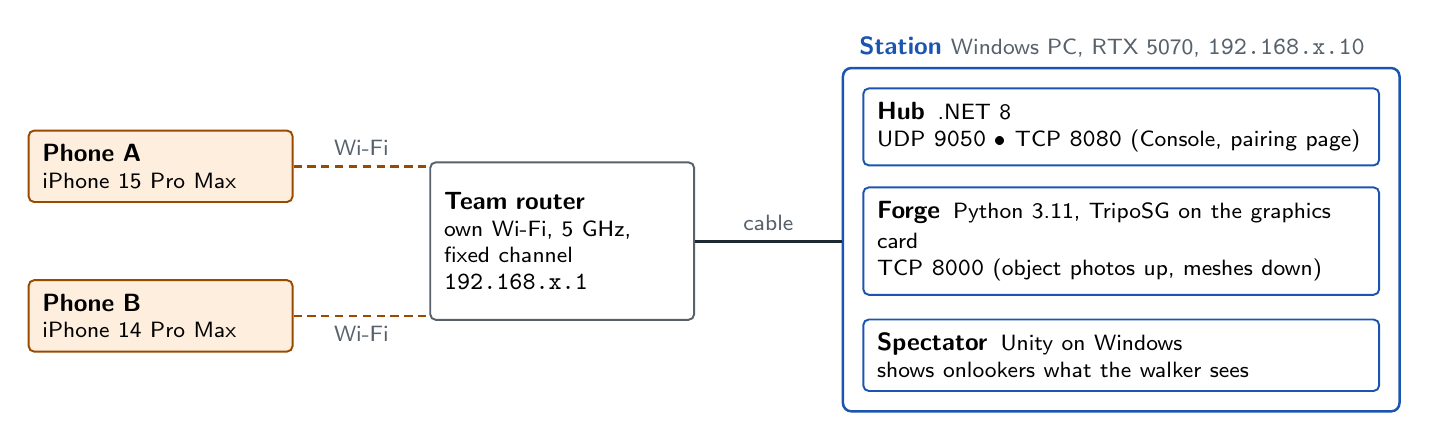
\begin{tikzpicture}[font=\small,
  box/.style={draw=#1,line width=0.7pt,rounded corners=2pt,align=left,inner sep=5pt},
  box/.default=rule]
  \node[box=accC,fill=laneC,text width=30mm] (pa) at (0,0.95) {\textbf{Phone A}\\[-0.5mm]{\footnotesize iPhone 15 Pro Max}};
  \node[box=accC,fill=laneC,text width=30mm] (pb) at (0,-0.95) {\textbf{Phone B}\\[-0.5mm]{\footnotesize iPhone 14 Pro Max}};
  \node[box=mute,fill=white,text width=30mm,minimum height=20mm] (rt) at (5.1,0)
    {\textbf{Team router}\\[-0.5mm]{\footnotesize own Wi-Fi, 5 GHz,}\\[-0.5mm]{\footnotesize fixed channel}\\[-0.5mm]{\footnotesize \code{192.168.x.1}}};
  \node[box=accD,fill=white,text width=62mm] (hub) at (12.2,1.45) {\textbf{Hub}\enskip{\footnotesize .NET 8}\\[-0.5mm]{\footnotesize UDP \code{9050} \textbullet{} TCP \code{8080} (Console, pairing page)}};
  \node[box=accD,fill=white,text width=62mm] (forge) at (12.2,0) {\textbf{Forge}\enskip{\footnotesize Python 3.11, TripoSG on the graphics card}\\[-0.5mm]{\footnotesize TCP \code{8000} (object photos up, meshes down)}};
  \node[box=accD,fill=white,text width=62mm] (spec) at (12.2,-1.45) {\textbf{Spectator}\enskip{\footnotesize Unity on Windows}\\[-0.5mm]{\footnotesize shows onlookers what the walker sees}};
  \node[draw=accD,line width=0.9pt,rounded corners=3pt,fit=(hub)(forge)(spec),inner sep=7pt,
        label={[font=\small\bfseries,text=accD,anchor=south west,xshift=1mm]north west:Station \textmd{\footnotesize\color{mute} Windows PC, RTX 5070, \code{192.168.x.10}}}] (st) {};
  \draw[line width=0.9pt,color=accC,dash pattern=on 3pt off 2pt] (pa.east) -- (rt.west |- pa.east) node[midway,above,font=\footnotesize,text=mute] {Wi-Fi};
  \draw[line width=0.9pt,color=accC,dash pattern=on 3pt off 2pt] (pb.east) -- (rt.west |- pb.east) node[midway,below,font=\footnotesize,text=mute] {Wi-Fi};
  \draw[line width=1.1pt,color=ink] (rt.east) -- (st.west |- rt.east) node[midway,above,font=\footnotesize,text=mute] {cable};
\end{tikzpicture}
\end{center}

\h{What this guide covers}
\begin{later}[Today and later.]
Parts 1 to 8 can be done today: the machine, the tools, the graphics card, the network and Unity.
Part 9 lists what to run once lane D has written the Hub, the Forge and the Spectator; none of that code exists yet.
\end{later}

\vspace{1mm}
{\small
\renewcommand{\arraystretch}{1.25}
\begin{tabular}{@{}>{\bfseries\color{accD}}r@{\hspace{3mm}}>{\bfseries\raggedright\arraybackslash}p{50mm}@{\hspace{3mm}}>{\raggedright\arraybackslash}p{110mm}@{}}
\toprule
 & Part & Done when\\
\midrule
1 & Prepare Windows & Windows is up to date, never sleeps on mains power, and you know whether its disk is encrypted\\
2 & Install the tools & Git, .NET 8, Python 3.11, the C++ compiler and the CUDA compiler each print their version\\
3 & Graphics driver & \code{nvidia-smi} names the RTX 5070\\
4 & Get the repository & \code{C:\textbackslash atlas\textbackslash station} holds \code{hub}, \code{forge} and \code{pipelines}\\
5 & PyTorch on the graphics card & The test prints \code{True} and the card's name. This is task \pid{P1-X03} of the plan\\
6 & TripoSG smoke test & One photo becomes a mesh on this card, also with no internet; seconds and video memory recorded\\
7 & Network & Both phones open a page served from the Station's fixed address (\pid{P1-X04}, the Station's half)\\
8 & Unity & The ATLAS project opens in Unity 6000.3.25f1\\
9 & When the code lands & Hub, Forge and Spectator run and a phone pairs\\
10 & Before every session & A checklist\\
11 & If something fails & A table of symptoms and fixes\\
\bottomrule
\end{tabular}}

\h{Before you start}
\begin{itemize}[leftmargin=5mm,itemsep=0.6mm,topsep=0mm]
\item \textbf{The PC:} Windows 11, 64-bit, an account with administrator rights, the monitor plugged into the RTX 5070.
      Keep 60 GB of disk free. The known downloads are PyTorch (3.3 GB), the CUDA Toolkit (3.4 GB) and the TripoSG
      weights (8.8 GB); the C++ compiler and Unity take several GB each.
\item \textbf{Internet} for Parts 1 to 6 and 8. The team router has none, so do those parts on a normal connection.
\item \textbf{For Part 7:} the team's router, a network cable and both phones.
\item \textbf{Accounts:} GitHub with access to the repository, and a Unity account.
\end{itemize}

\needspace{40mm}
\h{How to read the commands}
\begin{itemize}[leftmargin=5mm,itemsep=0.6mm,topsep=0mm]
\item Grey blocks are typed into PowerShell (the Terminal app). Copy them out of this PDF: they paste exactly as printed.
      A block of several lines can be pasted in one go; Terminal asks once whether to paste several lines.
\item \asadmin means a terminal opened with a right-click on the Start button\m Terminal (Admin).
\item In \code{192.168.x.10}, the first three numbers are your router's. Replace the \code{x} wherever it appears.
\item Two folders are used throughout: \cc!C:\atlas! (the repository) and \cc!C:\triposg! (the mesh generator).
\end{itemize}

% =====================================================================
\Part{Prepare Windows}{Windows is up to date, never sleeps on mains power, and you know whether its disk is encrypted.}
\begin{steps}
\step \act{Update Windows first.} Settings\m Windows Update: install everything and restart until nothing is pending.
      An update that arrives later restarts the PC in the middle of a session.

\step \act{Check the installer tool.} Part 2 uses \code{winget}.
\begin{cmd}
winget --version
\end{cmd}
      \see\ a version number. If the command is not found, run the line below and open a new terminal.
\begin{cmd}
Add-AppxPackage -RegisterByFamilyName -MainPackage Microsoft.DesktopAppInstaller_8wekyb3d8bbwe
\end{cmd}

\step \act{Allow long paths.} \asadmin Unity and Python packages make paths longer than the old Windows limit of 260 characters.
\begin{cmd}
$fs = "HKLM:\SYSTEM\CurrentControlSet\Control\FileSystem"
New-ItemProperty -Path $fs -Name LongPathsEnabled -Value 1 -PropertyType DWORD -Force
\end{cmd}

\step \act{Allow your own scripts to run.} Python environments are switched on by a script. Answer \code{Y}.
\begin{cmd}
Set-ExecutionPolicy -ExecutionPolicy RemoteSigned -Scope CurrentUser
\end{cmd}

\step \act{Never sleep on mains power.} \asadmin A sleeping PC stops the Hub and the Forge. A locked screen does not.
\begin{cmd}
powercfg /change standby-timeout-ac 0
powercfg /change hibernate-timeout-ac 0
powercfg /change monitor-timeout-ac 0
\end{cmd}
      Check in Settings\m System\m Power: sleep and screen-off read \emph{Never} when plugged in.

\step \act{See whether the disk is encrypted.} \asadmin The Hub will keep motion logs of walkers, which the plan treats as health data.
\begin{cmd}
manage-bde -status C:
\end{cmd}
      \see\ \code{Protection Status: Protection On}. If it reads \code{Off}, turn on Settings\m Privacy \& security\m
      Device encryption (named BitLocker on Windows Pro). If Windows offers neither, note it on the record sheet: the Hub's
      logs then go into an encrypted container before anyone from outside the team is logged.

\step \act{Restart the PC} so the long-path setting reaches every program.
\end{steps}

% =====================================================================
\Part{Install the tools}{the five checks in step 2.6 each print the line shown.}
\begin{steps}
\step \act{Git, .NET 8 and Python 3.11.} Answer \code{Y} to the agreement questions. Git for Windows brings Git LFS with it.
\begin{cmd}
winget install --id Git.Git -e
winget install --id Microsoft.DotNet.SDK.8 -e
winget install --id Python.Python.3.11 -e
\end{cmd}

\step \act{The C++ compiler.} It is needed once, in Part 6, to build one part of TripoSG. It must be the 2022 edition:
      the CUDA compiler of the next step does not accept Visual Studio 2026.
\begin{cmd}
$vs = "--passive --wait --norestart --add Microsoft.VisualStudio.Workload.VCTools --includeRecommended"
winget install --id Microsoft.VisualStudio.2022.BuildTools -e --override $vs
\end{cmd}

\step \act{The CUDA Toolkit 12.8.} It brings \code{nvcc}, the compiler for code that runs on the graphics card.
      PyTorch itself does not need it; the TripoSG build in Part 6 does. Download the installer (3.4 GB) and start it:
\begin{cmd}
$f = "cuda_12.8.1_572.61_windows.exe"
curl.exe -L -o $HOME\Downloads\$f https://developer.download.nvidia.com/compute/cuda/12.8.1/local_installers/$f
& "$HOME\Downloads\$f"
\end{cmd}
      Choose \emph{Custom (Advanced)} and untick everything except \emph{CUDA}. Above all, untick \emph{Driver components}:
      the installer carries driver 572.61, which is older than the first driver that lists the RTX 5070 (572.70), and it
      must not replace yours. For the same reason, do not use its Express option and do not install the toolkit through
      \code{winget}: both install every component.

\step \act{Unity Hub}, for Part 8.
\begin{cmd}
winget install --id Unity.UnityHub -e
\end{cmd}

\step \act{Restart the PC} if an installer asked for it. Otherwise close the terminal and open a new one, so it sees the new programs.

\step \act{Check all five.}
\begin{cmd}
git --version
git lfs version
dotnet --list-sdks
py -3.11 --version
nvcc --version
\end{cmd}
      \see
\begin{out}
git version 2.5x.x.windows.x
git-lfs/3.x.x (GitHub; windows amd64; go 1.xx)
8.0.4xx [C:\Program Files\dotnet\sdk]
Python 3.11.9
... Cuda compilation tools, release 12.8, V12.8.xx
\end{out}

\step \act{Set Git up for this user.}
\begin{cmd}
git config --global core.longpaths true
git lfs install
\end{cmd}
\end{steps}
\begin{trap}[Two traps.]
Typing \code{python} outside an environment may open the Microsoft Store: always type \code{py -3.11}.
If a newer .NET is already installed, keep it and install 8 as well; \code{dotnet --list-sdks} must list an \code{8.0} line.
\end{trap}

% =====================================================================
\Part{Graphics driver}{\code{nvidia-smi} names the RTX 5070 and shows a driver of 572.70 or newer.}
\begin{steps}
\step \act{Install the newest GeForce driver,} also when a driver is already there. Use the NVIDIA app, or
      \code{nvidia.com/drivers}: GeForce RTX 5070, Windows 11, Game Ready. Restart when it asks. Doing this after the
      CUDA Toolkit also puts things right if the toolkit's installer did replace the driver.

\step \act{Check the card.}
\begin{cmd}
nvidia-smi
\end{cmd}
      \see\ a table with \code{NVIDIA GeForce RTX 5070}, a \code{Driver Version} of 572.70 or higher, and about 12,000 MiB of memory.
      Write the driver version on the record sheet.

\step \act{Make a full graphics memory fail fast.} NVIDIA Control Panel\m Manage 3D settings\m Global Settings\m
      \emph{CUDA - Sysmem Fallback Policy}\m \emph{Prefer No Sysmem Fallback}\m Apply. Without it, a job that runs out of
      video memory carries on from system memory, many times slower, and reports no error.
\end{steps}

% =====================================================================
\Part{Get the repository}{\code{C:\textbackslash atlas\textbackslash station} holds \code{hub}, \code{forge} and \code{pipelines}.}
\begin{steps}
\step \act{Clone it to a short path.} A browser window asks you to sign in to GitHub the first time.
\begin{cmd}
git clone https://github.com/notwinston/StormHacks_2026_Blueberries.git C:\atlas
cd C:\atlas
git lfs pull
\end{cmd}

\step \act{Check.}
\begin{cmd}
dir C:\atlas\station
\end{cmd}
      \see\ three folders: \code{forge}, \code{hub}, \code{pipelines}.
\end{steps}

% =====================================================================
\Part{PyTorch on the graphics card}{the test prints \code{True} and the card's name. With .NET 8 from Part 2, that is task \pid{P1-X03} of the plan.}
\begin{steps}
\step \act{Make the Forge's Python environment.} The folder \code{.venv} is ignored by Git.
\begin{cmd}
cd C:\atlas\station\forge
py -3.11 -m venv .venv
.\.venv\Scripts\Activate.ps1
python -m pip install --upgrade pip setuptools wheel ninja
\end{cmd}
      \see\ the prompt now starts with \code{(.venv)}. Every later Python command needs that prefix: after opening a new
      terminal, run the third line again.

\step \act{Install PyTorch built for CUDA 12.8.} Use this line as printed. The chooser on \code{pytorch.org} no longer
      lists 12.8, and its older choice (12.6) does not support the 5070.
\begin{cmd}
pip install torch==2.7.1 torchvision==0.22.1 --index-url https://download.pytorch.org/whl/cu128
\end{cmd}

\step \act{Test it.}
\begin{cmd}
python -c "import torch; print(torch.__version__, torch.version.cuda, torch.cuda.is_available())"
python -c "import torch; print(torch.cuda.get_device_name(0), torch.cuda.get_device_capability(0))"
python -c "import torch; x = torch.rand(4000, 4000, device='cuda'); print(float((x @ x).mean()))"
\end{cmd}
      \see
\begin{out}
2.7.1+cu128 12.8 True
NVIDIA GeForce RTX 5070 (12, 0)
a number close to 1000, and no warning
\end{out}
\end{steps}
\begin{trap}
A version that ends in \code{+cpu}, \code{False}, or a warning that \code{sm\_120 is not compatible} all mean the wrong
build was installed. Remove it and repeat step 5.2 exactly, including \code{--index-url}:
\begin{cmd}
pip uninstall -y torch torchvision
\end{cmd}
\end{trap}

% =====================================================================
\Part{TripoSG smoke test}{one photo becomes a mesh of about 5,000 triangles on this card, also with the network unplugged, and the seconds and the peak video memory are on the record sheet.}
\begin{later}[Why this part matters.]
TripoSG is the generator inside the Forge. One of its parts, \code{diso}, has no ready-made Windows build and is compiled
on this PC in step 6.3. Nobody has reported that build on an RTX 50 card, so this is the step most likely to fail.
The plan marks it ``verify''; this part is that check, and it also measures the seconds per object the plan still lacks.
\end{later}
\begin{steps}
\step \act{Get TripoSG at the pinned version,} outside the repository.
\begin{cmd}
git clone https://github.com/VAST-AI-Research/TripoSG.git C:\triposg
cd C:\triposg
git checkout fc5c40990181e2a756c4e0b1c2f4d6b5202faf8c
\end{cmd}

\step \act{Install its Python packages} into the environment of Part 5 (the prompt shows \code{(.venv)}). Do not use
      TripoSG's own \code{requirements.txt}: it asks for a NumPy that has no Python 3.11 build, and it leaves packages out.
      These are the versions of April 2025, when TripoSG was last changed; newer ones break it.
\begin{cmd}
pip install numpy==1.26.4 scipy==1.17.1 scikit-image==0.26.0 opencv-python==4.11.0.86
pip install diffusers==0.32.2 transformers==4.51.1 huggingface_hub==0.30.2 tokenizers==0.21.1 safetensors==0.5.3
pip install peft==0.15.1 accelerate==1.6.0 einops==0.8.2 omegaconf==2.3.1 trimesh==4.12.2
pip install jaxtyping==0.3.11 typeguard==4.6.0 pymeshlab==2025.7.post1
pip check
python -c "import torch; print(torch.__version__)"
\end{cmd}
      \see\ \code{No broken requirements found.} and then \code{2.7.1+cu128}: PyTorch is still the build of Part 5.

\step \act{Build \code{diso}.} This runs the C++ compiler and \code{nvcc} from Part 2. Use a normal PowerShell
      window, not a Visual Studio developer prompt. The first three lines point the build at the 12.8 toolkit and at the
      5070.
\begin{cmd}
$env:CUDA_HOME = "C:\Program Files\NVIDIA GPU Computing Toolkit\CUDA\v12.8"
$env:FORCE_CUDA = "1"
$env:TORCH_CUDA_ARCH_LIST = "12.0"
pip install diso==0.1.4 --no-build-isolation --no-cache-dir
python -c "import torch; from diso import DiffDMC; print('diso ok')"
\end{cmd}
      \see\ \code{Successfully installed diso-0.1.4}, then \code{diso ok}.

\step \act{First run.} It downloads 8.8 GB of weights into \cc!C:\triposg\pretrained_weights!, once.
\begin{cmd}
$img = "assets/example_data/hjswed.png"
python -m scripts.inference_triposg --image-input $img --output-path out.glb
\end{cmd}
      \see\ \code{Mesh saved to out.glb} as the last line.

\step \act{Timed run with the triangle limit.} First start this in a second terminal and leave it running; it prints the
      video memory in use once a second.
\begin{cmd}
nvidia-smi --query-gpu=memory.used,memory.total --format=csv -l 1
\end{cmd}
      Then paste these three lines together in the first terminal. The last one prints the seconds.
\begin{cmd}
$t = Get-Date
python -m scripts.inference_triposg --image-input $img --faces 5000 --output-path out_5000.glb
((Get-Date) - $t).TotalSeconds
\end{cmd}
      Write down the seconds and the highest memory figure. The time includes loading the model, which the Forge does only once.

\step \act{Check the mesh.}
\begin{cmd}
python -c "import trimesh; m = trimesh.load('out_5000.glb', force='mesh'); print(len(m.faces), m.extents)"
\end{cmd}
      \see\ a count of about 5000, then three sizes. To look at it, drag the file into a glTF viewer in the browser, for
      example \code{sandbox.babylonjs.com}: it must be a recognisable object.

\step \act{Run it with no internet.} Pull the network cable or turn Wi-Fi off, then:
\begin{cmd}
$env:HF_HUB_OFFLINE = "1"
python -m scripts.inference_triposg --image-input $img --faces 5000 --output-path out_offline.glb
\end{cmd}
      It must finish as before, with no download. The demo runs on a router with no internet.

\step \act{Save what worked,} then commit the file: it is the first version of the Forge's lock file.
\begin{cmd}
pip freeze | Set-Content C:\atlas\station\forge\requirements.lock.txt
\end{cmd}
\end{steps}
\begin{trap}[If this part fails.]
Copy the first error line and give it to lane D; Part 11 lists the known ones. The ways out, in order: rebuild
\code{diso} in a fresh environment; run TripoSG without \code{diso} on its slower built-in surface extraction (a small
code change, untested); run the Forge under WSL2; use the hosted service of open item 8, or the built-in furniture set.
The app does not depend on the Forge.
\end{trap}
\begin{later}[For lane D.]
\textbf{Licences:} TripoSG is MIT, but \code{diso} is CC BY-NC 4.0 and TripoSG's own background remover (RMBG-1.4) is
non-commercial. Enter all three in the licence ledger. \textbf{Background removal:} the current \code{rembg} needs NumPy
2.3 or newer, which clashes with the set above, and its default model is now the non-commercial \code{bria-rmbg}; name
the model (\code{u2net}) and settle NumPy in the lock file. \textbf{Working folder:} TripoSG looks for
\code{pretrained\_weights} under the folder it is started from, so the Forge must start it from \cc!C:\triposg!.
\textbf{Versions:} do not upgrade the set of step 6.2; \code{transformers} 4.57 and newer stop TripoSG from loading.
\end{later}

% =====================================================================
\Part{Network}{both phones open the Station's test page at its fixed address, on port 8080 and on port 8000. That is the Station's half of task \pid{P1-X04}.}
\begin{steps}
\step \act{Set the router up, once.} Give it a Wi-Fi name and password of your own. On the 5 GHz band, fix the channel:
      36, 40, 44, 48, 149, 153, 157 or 161. Never ``Auto'', and never a channel from 52 to 144, which the router must
      leave when it detects radar. Set the channel width to 20 MHz: the link needs little bandwidth and a narrow channel
      is steadier in a crowded hall. Channel 44 or 149 is the best pick, because the phones' own AirDrop radio rests there.
      The router needs no internet cable.

\step \act{Cable the PC to the router} (a LAN port) and read the adapter's name, its address and its hardware address.
\begin{cmd}
Get-NetAdapter -Physical | Format-Table Name, Status, MacAddress, LinkSpeed
Get-NetIPAddress -AddressFamily IPv4 | Format-Table InterfaceAlias, IPAddress
\end{cmd}
      The wired adapter is usually named \code{Ethernet}. If yours differs, use your name in the commands below.

\step \act{Give the Station the fixed address \code{192.168.x.10}.} In the router's own page, reserve that address for
      the hardware address you just read (the setting is called DHCP reservation or static lease). Then:
\begin{cmd}
ipconfig /renew
ipconfig
\end{cmd}
      \see\ \code{IPv4 Address . . . : 192.168.x.10} under the wired adapter.

\step \act{Mark the network as private.} \asadmin Windows blocks incoming connections on a network it calls public.
\begin{cmd}
Get-NetConnectionProfile
Set-NetConnectionProfile -InterfaceAlias "Ethernet" -NetworkCategory Private
\end{cmd}

\step \act{Open the three ports.} \asadmin These are the plan's three firewall rules, limited to private networks.
\begin{cmd}
$allow = @{ Direction = "Inbound"; Action = "Allow"; Profile = "Private" }
New-NetFirewallRule @allow -DisplayName "ATLAS Hub UDP" -Protocol UDP -LocalPort 9050
New-NetFirewallRule @allow -DisplayName "ATLAS Hub HTTP" -Protocol TCP -LocalPort 8080
New-NetFirewallRule @allow -DisplayName "ATLAS Forge" -Protocol TCP -LocalPort 8000
Get-NetFirewallRule -DisplayName "ATLAS*" | Format-Table DisplayName, Enabled, Direction, Action, Profile
\end{cmd}
      \see\ three rows, each \code{True}, \code{Inbound}, \code{Allow}, \code{Private}.

\step \act{Serve a test page.} If Windows asks whether Python may be reached from networks, allow private networks only.
\begin{cmd}
mkdir C:\atlas-test
cd C:\atlas-test
Set-Content index.html "<h1>ATLAS Station is reachable</h1>"
py -3.11 -m http.server 8080 --bind 0.0.0.0
\end{cmd}

\step \onphone Join the team's Wi-Fi. iOS notices that it has no internet and may offer to use mobile data: decline and
      stay on the Wi-Fi. Open Safari at \code{http://192.168.x.10:8080}.
      \see\ the heading \emph{ATLAS Station is reachable}.

\step \act{Repeat for the Forge's port.} Stop the server with Ctrl+C, start it on 8000, and open
      \code{http://192.168.x.10:8000} on both phones.
\begin{cmd}
py -3.11 -m http.server 8000 --bind 0.0.0.0
\end{cmd}
      Stop it with Ctrl+C when both phones have shown the page. The UDP port 9050 cannot be tested with a browser; it is
      proven when the Hub runs (Part 9).

\step \onphone Before every session: Settings\m General\m AirDrop\m Receiving Off, and Settings\m General\m AirPlay \&
      Continuity\m Handoff off. Both make the phone's radio hop channels, which shows as stutter on the link.
\end{steps}
\begin{trap}[If the PC loses its internet when the router is cabled:]
Windows prefers the cable, and the team router leads nowhere. This happens when the PC also uses Wi-Fi on another network
for its internet. In an administrator terminal, make the cable the last choice, then check that downloads work again.
\begin{cmd}
Set-NetIPInterface -InterfaceAlias "Ethernet" -AddressFamily IPv4 -InterfaceMetric 500
\end{cmd}
\end{trap}
\begin{trap}[If the router cannot reserve addresses:]
set the address on the PC instead, in an administrator terminal, with your router's numbers in place of \code{x}.
Pick an address outside the range the router hands out by itself.
\begin{cmd}
New-NetIPAddress -InterfaceAlias "Ethernet" -IPAddress 192.168.x.10 -PrefixLength 24
\end{cmd}
\end{trap}

% =====================================================================
\Part{Unity}{the ATLAS project opens in Unity 6000.3.25f1 with no red error in its Console window.}
\begin{steps}
\step \act{Open Unity Hub and sign in} with your Unity account. If the Hub shows no licence, add the free Personal one
      (account menu\m Manage licenses\m Add).

\step \act{Install exactly the project's Editor version.} This opens the Hub's install dialog for that version.
\begin{cmd}
Start-Process "unityhub://6000.3.25f1/e1dba0a9aba4"
\end{cmd}
      Building for Windows needs no extra module, so every optional box can stay unticked. If the link does nothing:
      Hub\m Installs\m Install Editor\m Archive, and pick 6000.3.25f1 there.

\step \act{Register Git LFS and Unity's merge tool for this clone.} The script needs the Editor of the step before.
\begin{cmd}
cd C:\atlas
& "C:\Program Files\Git\bin\bash.exe" tools/setup_git.sh
\end{cmd}
      \see\ \code{Git LFS and UnityYAMLMerge (6000.3.25f1) are set up for this clone.}

\step \act{Open the project.} Hub\m Add\m Add project from disk\m \cc!C:\atlas\ATLAS!, then open it with 6000.3.25f1.
      If the Hub proposes another Editor version, cancel: a different version rewrites project files. The first opening
      imports every asset.

\step \act{Check.} Window\m General\m Console shows no red error. If it does, send the first one to lane A: the project
      has not been opened on Windows before.
\end{steps}

% =====================================================================
\Part{When the code lands}{the Hub, the Forge and the Spectator run, and a phone pairs by QR code.}
\begin{later}
Nothing in this part can be done today. The Hub, the Forge service and the Spectator are tasks \pid{P1-D02},
\pid{P1-D08} and \pid{P1-D05} of lane D. The commands below are the plan's (Appendix C.7); when a folder has a README,
the README wins.
\end{later}
\begin{steps}
\step \act{Hub.} It listens on UDP 9050 and serves the Console on TCP 8080.
\begin{cmd}
cd C:\atlas
dotnet run --project station/hub
\end{cmd}
      Open \code{http://localhost:8080} for the Console. If the Hub prints \code{no packets received} ten seconds after a
      phone tried to connect, the firewall or the network category is wrong: steps 7.4 and 7.5.

\step \act{Forge.} Start it from the environment of Part 5, after installing the Forge's lock file.
\begin{cmd}
cd C:\atlas\station\forge
.\.venv\Scripts\Activate.ps1
uvicorn forge.app:app --host 0.0.0.0 --port 8000
\end{cmd}
      Open \code{http://localhost:8000/health}. It reports \code{ok}, \code{gpu}, \code{queue}, \code{pipelineVer} and
      \code{debugKeep}. \code{debugKeep} must be \code{false} whenever someone from outside the team is scanned: it
      means object photos are kept on disk.

\step \act{Pair a phone.} Open \code{http://localhost:8080/pair} on the Station: it shows a QR code. Scan it with the
      phone's Camera app. The app asks once for permission to use the local network: allow it, with the phone in your hand.

\step \act{Spectator.} Run the Unity Editor in play mode, or the Windows build made with the \code{ATLAS\_SPECTATOR}
      symbol. It joins the Hub as a spectator.

\step \act{Logs.} The Hub's \code{logs} folder must sit on the encrypted disk of step 1.6.

\step \act{One program owns the graphics card.} The Forge runs one job at a time. Do not run the TripoSG test of Part 6
      while the Forge is up, and close other programs that use video memory.

\step \act{Lung data pipeline.} \code{station/pipelines} has its own environment and README; it is being written on the
      branch \code{p2-lung-data}.
\end{steps}

% =====================================================================
\Part{Before every session}{every box is ticked.}
\begin{multicols}{2}
\small
\cb The PC is on mains power and does not sleep (step 1.5).\par\vspace{1.2mm}
\cb Windows Update shows nothing pending, and updates are paused (Settings\m Windows Update\m Pause).\par\vspace{1.2mm}
\cb Do Not Disturb is on (Settings\m System\m Notifications).\par\vspace{1.2mm}
\cb The cable goes to the team router; \code{ipconfig} shows \code{192.168.x.10}; the network is Private (step 7.4).\par\vspace{1.2mm}
\cb The router is on its fixed channel.\par\vspace{1.2mm}
\cb With no internet: \cc!$env:HF_HUB_OFFLINE = "1"! is set in the terminal that starts the Forge.\par\vspace{1.2mm}
\cb Started in this order: Hub, Forge, Spectator, then the Console in the browser.\par\vspace{1.2mm}
\cb \code{/health} reports \code{ok}, and \code{debugKeep} is \code{false}.\par\vspace{1.2mm}
\cb \code{nvidia-smi} shows little video memory in use before the first job.\par\vspace{1.2mm}
\cb Both phones: on the team Wi-Fi, AirDrop and Handoff off, link dot green.\par\vspace{1.2mm}
\cb Everyone knows the rule: if the Station fails, carry on. The app is complete without it and the furniture falls back
    to the built-in set.\par
\end{multicols}

% =====================================================================
\Part{If something fails}{}
{\small
\renewcommand{\arraystretch}{1.3}
\begin{tabular}{@{}>{\raggedright\arraybackslash}p{55mm}@{\hspace{4mm}}>{\raggedright\arraybackslash}p{50mm}@{\hspace{4mm}}>{\raggedright\arraybackslash}p{65mm}@{}}
\toprule
\textbf{Symptom} & \textbf{Cause} & \textbf{Fix}\\
\midrule
\code{winget} is not recognised & App Installer is not registered yet & Step 1.2\\
\code{Activate.ps1}: running scripts is disabled & PowerShell's default policy & Step 1.4\\
\code{python} opens the Microsoft Store & A Windows alias stands in for Python & Type \code{py -3.11}, or activate the environment first\\
The PyTorch version ends in \code{+cpu}, or the test prints \code{False} & The plain build was installed & Uninstall it and repeat step 5.2 with \code{--index-url}\\
Warning: \code{sm\_120 is not compatible} & A build for CUDA 12.6 or older & The same\\
\code{diso}: Microsoft Visual C++ 14.0 or greater is required & The C++ compiler is missing, or this terminal is older than its install & Step 2.2, then a new terminal. Still failing: open the Visual Studio Installer and tick \emph{Desktop development with C++}\\
\code{diso}: the VC environment is activated but \code{DISTUTILS\_USE\_SDK} is not set & The build was started from a Visual Studio developer prompt & Use a normal PowerShell window\\
\code{diso}: invalid command \code{bdist\_wheel} & The \code{wheel} package is missing & The fourth line of step 5.1\\
\code{diso}: the detected CUDA version mismatches the version used to compile PyTorch & Another CUDA Toolkit was found first & Check that the folder in the first line of step 6.3 exists; install the 12.8 toolkit (step 2.3)\\
\code{diso}: \code{nvcc} reports an unsupported Visual Studio version & Visual Studio 2026 is installed & Install the 2022 Build Tools of step 2.2 and remove 2026\\
\code{diso}: No module named torch, during the build & \code{--no-build-isolation} was left out & Repeat step 6.3 as printed\\
TripoSG ends with \code{'NoneType' object has no attribute 'astype'} & \code{diso} failed on the graphics card; the real error is the \code{CUDA error} line printed above it & \code{pip uninstall -y diso}, then step 6.3 in a new terminal. If it comes back, give that line to lane D\\
TripoSG: unexpected keyword argument \code{offload\_state\_dict} & A newer \code{transformers} was installed & Repeat the second line of step 6.2\\
\code{DLL load failed while importing \_C} & \code{diso} was built against another PyTorch or CUDA & Delete \code{.venv}, redo Part 5 and steps 6.2 and 6.3\\
No module named \code{triposg}, or the weights download again & TripoSG was started from the wrong folder & \cc!cd C:\triposg! and use \code{python -m scripts.inference\_triposg}\\
TripoSG is very slow and prints no error & Video memory is full and Windows spilled into system memory & Step 3.3; close Unity and browsers; watch \code{nvidia-smi}\\
A phone cannot open the test page & The network is Public, a rule is missing, the address is wrong, or the phone left the Wi-Fi & Steps 7.3 to 7.5; on the phone, check it is still on the team Wi-Fi\\
The PC lost its internet when the router was cabled & Windows prefers the cable & The first box after step 7.9\\
A phone never connects to the Hub & In this order: the local-network permission was refused; a firewall rule is missing; the server listens on \code{localhost} only & Phone: Settings\m Privacy \& Security\m Local Network\m ATLAS on. PC: step 7.5. Server: it must listen on \code{0.0.0.0}\\
Unity Hub proposes another Editor version & The exact version is not installed & Cancel; step 8.2\\
Pink or missing assets in Unity & The large files were not fetched & \code{git lfs pull} in \cc!C:\atlas!\\
The Hub and the Forge stopped by themselves & The PC went to sleep & Step 1.5\\
\bottomrule
\end{tabular}}

% =====================================================================
\h{Record sheet}
Fill this in as you go, then copy it into \code{docs/versions.md} under ``Station PC''. The plan asks for the installed
numbers, and two of them are still open questions: whether TripoSG runs on this card, and how long one object takes.

\vspace{2mm}
{\small
\renewcommand{\arraystretch}{1.75}
\begin{tabular}{@{}>{\raggedright\arraybackslash}p{54mm}p{26mm}@{\hspace{7mm}}>{\raggedright\arraybackslash}p{54mm}p{26mm}@{}}
Windows edition and version & \fillin{25mm} & PyTorch and torchvision & \fillin{25mm}\\
Disk encrypted (step 1.6) & \fillin{25mm} & TripoSG commit (first 8 characters) & \fillin{25mm}\\
GeForce driver & \fillin{25mm} & \code{diso} built and imported & \fillin{25mm}\\
.NET SDK & \fillin{25mm} & Seconds for one object, 5,000 triangles & \fillin{25mm}\\
Python & \fillin{25mm} & Peak video memory (MiB) & \fillin{25mm}\\
C++ Build Tools & \fillin{25mm} & Ran with no internet & \fillin{25mm}\\
CUDA Toolkit (\code{nvcc}) & \fillin{25mm} & Station address & \fillin{25mm}\\
Unity Editor & \fillin{25mm} & Router channel and width & \fillin{25mm}\\
Both phones opened port 8080 and 8000 & \fillin{25mm} & Date, and who did it & \fillin{25mm}\\
\end{tabular}}

\end{document}
